%%
%% This is file `main_template_based.tex',
%% derived directly from the official ACM proceedings template `sigconf.tex'.
%%
%% --------------------------------------------------------------------------
%% Official ACM Template Directives (from sigconf.tex)
%% --------------------------------------------------------------------------
%% Commands for TeXCount
%TC:macro \cite [option:text,text]
%TC:macro \citep [option:text,text]
%TC:macro \citet [option:text,text]
%TC:envir table 0 1
%TC:envir table* 0 1
%TC:envir tabular [ignore] word
%TC:envir displaymath 0 word
%TC:envir math 0 word
%TC:envir comment 0 0
%%
%% The first command in your LaTeX source must be the \documentclass command.
\documentclass[sigconf]{acmart}

%%
%% \BibTeX command to typeset BibTeX logo in the docs
\AtBeginDocument{%
  \providecommand\BibTeX{{%
    Bib\TeX}}}

%%
%% Rights management information.
%% These commands have sample values in sigconf.tex; they are kept commented out
%% pending completion and receipt of the official ACM e-Rights form by the authors.
%%\setcopyright{acmlicensed}
%%\copyrightyear{2026}
%%\acmYear{2026}
%%\acmDOI{XXXXXXX.XXXXXXX}

%%
%% These commands are for a PROCEEDINGS abstract or paper.
\acmConference[ICEFronT 2026]{2026 International Conference on Evolutionary Frontier Technologies}{November 2026}{Cox's Bazar, Bangladesh}
%%\acmBooktitle{ICEFronT 2026: Proceedings of the 2026 International Conference on Evolutionary Frontier Technologies, November 2026, Cox's Bazar, Bangladesh}
%%\acmISBN{978-1-4503-XXXX-X/2026/11}

%%
%% Submission ID from organizers
\acmSubmissionID{929}

%%
%% end of the preamble, start of the body of the document source.
\begin{document}

%%
%% The "title" command has an optional parameter,
%% allowing the author to define a "short title" to be used in page headers.
\title{Attention-Guided YOLOv11 for Object Detection in Unstructured Bangladeshi Traffic}

%%
%% The "author" command and its associated commands are used to define
%% the authors and their affiliations.
\author{Md. Taher Bin Omar Hijbullah}
\affiliation{%
  \institution{International University of Business Agriculture and Technology (IUBAT)}
  \country{Bangladesh}
}
\email{hijbullah119445@gmail.com}

\author{Md. Rony Mia}
\affiliation{%
  \institution{International University of Business Agriculture and Technology (IUBAT)}
  \country{Bangladesh}
}
\email{ronyarif800@gmail.com}

\author{Mahedi Hasan}
\affiliation{%
  \institution{International University of Business Agriculture and Technology (IUBAT)}
  \country{Bangladesh}
}
\email{mahedi.cse@iubat.edu}

\author{Hasibur Rahman}
\affiliation{%
  \institution{International University of Business Agriculture and Technology (IUBAT)}
  \country{Bangladesh}
}
\email{inbox.hasibur.rahman@gmail.com}

\author{Ferdaus Anam Jibon}
\affiliation{%
  \institution{International University of Business Agriculture and Technology (IUBAT)}
  \country{Bangladesh}
}
\email{jibon.cse@iubat.edu}

%%
%% The abstract is a short summary of the work to be presented in the article.
\begin{abstract}
In the South Asian context, traffic is complex and chaotic due to high population density, unstructured roads, and diverse types of transport. Vision-based systems face substantial challenges here due to extreme visual occlusion, a wide variety of unpredictable vehicle shapes, and erratic environments. Standard real-time object detection models are mostly trained on structured datasets from developed countries, which fail to generalize to this region. This makes them less useful for Advanced Driver Assistance Systems (ADAS). We propose a modified YOLOv11 architecture integrated with attention modules capable of handling complex backgrounds and dense traffic. Our model uses the Convolutional Block Attention Module (CBAM) injected specifically into the P5 feature map to improve core feature extraction capabilities in these complex environments. To train the model, we curated a custom dataset of 265,698 annotated instances sourced from the Mendeley Bangladeshi Traffic Flow, Dhaka-AI, and Poribohon-BD datasets to focus on non-standard local vehicles like rickshaws and CNGs. Our 50-epoch experiments show that baseline YOLOv11m achieved 75.1\% mAP@50, while the optimized CBAM model improved performance to 75.7\% mAP@50 on the validation set, maintaining real-time inference ($\sim$4.7~ms/frame). The attention mechanism excelled on complex vehicles, achieving 90.8\% mAP@50 for the Rickshaw class and boosting truck detection by 1.5 percentage points. Error analysis reveals that the architecture is highly sensitive to extreme data imbalance, especially for minority classes like cycles. Qualitative evaluation and error analysis show that the lack of data remains the main bottleneck for detecting minority classes in intelligent transportation networks.
\end{abstract}

%%
%% The code below is generated by the tool at http://dl.acm.org/ccs.cfm.
%% NOTE: Pending author review and approval. Kept commented out.
%%\begin{CCSXML}
%%<ccs2012>
%% <concept>
%%  <concept_id>10010147.10010178.10010224.10010245.10010250</concept_id>
%%  <concept_desc>Computing methodologies~Object detection</concept_desc>
%%  <concept_significance>500</concept_significance>
%% </concept>
%%</ccs2012>
%%\end{CCSXML}
%%
%%\ccsdesc[500]{Computing methodologies~Object detection}

%%
%% Keywords. Separate the keywords with commas.
\keywords{Object Detection, YOLOv11, Convolutional Block Attention Module, Advanced Driver Assistance Systems, Unstructured Traffic, Deep Learning}

%%
%% This command processes the author and affiliation and title
%% information and builds the first part of the formatted document.
\maketitle
\section{Introduction}
In the modern era, transportation systems lean towards Intelligent Transportation Systems (ITS) and Advanced Driver Assistance Systems (ADAS), which require real-time cameras and object detectors. Standard Western datasets like KITTI\cite{1a}, Cityscapes\cite{2a}, or COCO\cite{3a} fail to represent the reality of Dhaka traffic due to unstructured streets, unpredictable pedestrians, diverse vehicle shapes, and severe visual occlusion. In addition, non-motorized and custom-built vehicles like rickshaws, CNGs, auto-rickshaws, and easy-bikes do not exist in standard benchmarks \cite{Hasan2021VehicleClassification}. To provide reliable collision warnings in ADAS, vision systems must recognize these specific vehicle shapes, but standard models do not adequately represent these regional classes and struggle to detect them. Another major challenge is that in dense traffic, vehicles frequently overlap and occlude one another, making it difficult for feature extractors to separate vehicle boundaries from cluttered backgrounds. To improve feature extraction under these conditions, we integrate the Convolutional Block Attention Module (CBAM)\cite{Woo2018CBAM} into YOLOv11m, helping the network emphasize informative spatial and channel features in complex scenes. We curated a custom dataset based on the Bangladeshi Traffic Flow Dataset from Mendeley Data\cite{Islam2025BangladeshiTrafficFlow} along with regional sources to focus on local vehicles. The evaluation achieved 90.8\% mAP@50 for the visually complex Rickshaw class on Bangladeshi roads.
Overall, our main contributions are:
\begin{enumerate}
    \item We curated and standardized a custom dataset from regional traffic sources, unifying annotations to represent local vehicle classes in complex Bangladeshi traffic.
    \item We integrated CBAM into the deep layers of the YOLOv11m architecture to handle heavy visual occlusion in unstructured traffic scenes.
    \item We evaluated the computational performance of the model on an NVIDIA Tesla T4 GPU, achieving an inference latency of approximately 4.7~ms per frame.
    \item We conducted a qualitative failure analysis and examined class-wise performance disparities, showing that architectural modification alone does not fully resolve extreme dataset imbalance in this study.
\end{enumerate}
The paper reviews related work in Section II and Section III shows the proposed CBAM-integrated YOLOv11 architecture. Sections IV and VII cover the dataset, experimental setup, and performance analysis, and  Section VIII concluding remarks and future work.

\section{RELATED WORK}

\subsection{Evolution of Real-Time Object Detection}

For the past few years, object detection relied on heavy, two-stage networks, but everything changed when Redmon et al. introduced the original YOLO (You Only Look Once) architecture\cite{redmon2016you}. The YOLO family has evolved rapidly over the last few years with new versions and improvements. Recently, Jocher et al. advanced YOLO further with YOLOv11, reducing parameter counts\cite{Jocher2025YOLOv11} and improving deep feature extraction through novel C3k2 modules and C2PSA attention mechanisms\cite{9a}. However, a fundamental challenge remains in YOLO architectures as they struggle with unstructured data. Zhang et al. observe in comparative studies that baseline YOLOv11 models face limitations in detecting highly occluded or structurally complex small objects\cite{zhang2025trinext}. When YOLOv11 is deployed in dense, overlapping clusters of vehicles, recall drops significantly because the baseline cannot separate highly occluded bounding boxes without architectural modification.

\subsection{Attention Mechanisms in Computer Vision}
When a neural network gets very deep it often loses fine details of small or partially hidden objects. To fix this issue, an attention mechanism was introduced to guide the network “where” and “what” to focus on such as the Squeeze-and-Excitation (SE) network by Hu et al., which effectively captured channel importance, but ignored spatial location information entirely \cite{11a}. To overcome this limitation, Woo et al. introduce (CBAM) Convolutional Block Attention Module \cite{Woo2018CBAM}, which achieves better attention by applying channel attention first, then spatial attention sequentially. Recently, integration of CBAM into the YOLOv11 backbone has become a key research focus for handling complex environments. In July 2025, Garshasebi et al.\cite{garshasebi2025improving} integrated CBAM into YOLOv11 for remote sensing imagery, achieving a mean Average Precision (mAP@50) of 76.68\% by focusing on critical regions and reducing background noise. Also Khan et al. applied YOLOv11 with CBAM for pipeline defect detection and got accuracy improvements compared to the baseline model\cite{khan2025pipeline}. These studies prove CBAM is very effective at extracting weak geometric features from noisy backgrounds and highlights important features even when objects overlap in dense and cluttered scenes.

\subsection{Perception in Unstructured Traffic (The South Asian Context)}
When it comes to intelligent transportation in developing regions, the research is still catching up. In Bangladeshi perspective, traffic in cities like Dhaka, Gazipur is chaotic and unstructured which do not include native vehicles like rickshaws or CNGs in standard Western datasets. The challenges early attempts face is they struggled with unstructured traffic detection. For example, in 2021 study by Rahman et al.\cite{rahman2021densely} using an ensemble of YOLOv5 models on the Dhaka-AI dataset and reached mAP of only 45.8\% which shows the extreme difficulty of detecting traffic in such conditions. Recently, the open-source community has provided better datasets, such as the Bangladeshi Traffic Flow Dataset by Islam et al. \cite{Islam2025BangladeshiTrafficFlow}. In 2022, Rahman et al.\cite{rahman2022fine} fine-tuned deep convolutional networks to classify native Bangladeshi vehicles with improved accuracy. Hossain et al.\cite{17a} analyzed the conditions of rickshaw pullers in Dhaka city and highlighted the significant presence of non-motorized transport in urban traffic environments. Earlier studies usually treat deep learning models as black boxes, using transfer learning without fixing the mathematical cause of bounding box suppression in dense traffic. Our research differ from those earlier studies by building on regional datasets but go beyond simple retraining. We actively modify the YOLOv11 architecture instead of just applying transfer learning by injecting CBAM directly into the deep feature layers which target the extreme occlusion issues in South Asian traffic across a full, 9-class unstructured environment.

\section{MATHEMATICAL FORMULATION AND PROPOSED ARCHITECTURE}
We discovered several mathematical limits of the YOLOv11 in chaotic contexts by analyzing the baseline model. We address these by introducing a spatial and channel attention mechanism. 


\subsection{Baseline YOLOv11 Formulation}

YOLOv11 identifies objects in the images by predicting the position of objects by identifying the bounding boxes using learnt visual features. Nevertheless, it is difficult to detect in the most congested areas like Dhaka because of heavy traffic and obscuring objects, whereby cars usually come between the lens and the captured objects. In order to overcome this challenge, the base model uses Complete Intersection over Union (CIoU) loss that bounds box regression by taking into consideration the overlap, center distance, and aspect ratio consistency of the predicted and ground-truth boxes.. The CIoU loss is defined as:

\begin{equation}
L_{CIoU} = 1 - IoU + \frac{\rho^2(b, b_{gt})}{c^2} + \alpha \nu
\end{equation}


\subsection{Convolutional Block Attention Module (CBAM)}
The baseline model has a limitation during the deep feature extraction stage. When a bus occludes the lower part of a car, the feature extraction process may confuse the remaining visible features with background information, which can lead to missed detections. To address this issue, we incorporate the Convolutional Block Attention Module (CBAM)\cite{Woo2018CBAM}, which helps the model focus on more informative features..

CBAM forces the network to calculate "What is important?" (Channel Attention) and "Where is it?" (Spatial Attention). When an intermediate feature map $F \in \mathbb{R}^{C \times H \times W}$, CBAM sequentially generates a 1D channel attention map $M_{c}$ and a 2D spatial attention map $M_{s}$. The sequential attention process is formulated as:
\[
F' = M_{c}(F) \otimes F
\]
\[
F'' = M_{s}(F') \otimes F'
\]


(where $\otimes$ denotes element-wise multiplication).

\begin{enumerate}
    \item \textbf{Channel Attention:} At the channel attention stage, spatial information from the feature map is compressed using both average pooling and max pooling. These pooled features are then passed through a shared Multi-Layer Perceptron (MLP), which learns the importance of each channel.
    
    \item \textbf{Spatial Attention:} In the spatial attention stage, the channel-refined feature map $F'$ is first pooled along the channel dimension and then processed using a convolution layer with a $7 \times 7$ kernel. The larger receptive field allows the model to capture broader spatial relationships within the scene, and this approach helps the model to detect objects that are partially hidden, such as pedestrians standing close to large buses.

\end{enumerate}


\subsection{Architectural Integration Strategy}
Rather than adding the attention mechanism to the detection head, we designed a custom \texttt{ULTIMATE\_CBAM} module and injected it within the YOLOv11m backbone.

In our implementation, we replace the block at Layer~23 with the CBAM module to intercept the $P5$ feature map before features are forwarded to the detection head (Fig.~\ref{fig:arch}). In YOLOv11m, the width multiplier is set to $1.00$, so the $P5$ layer operates with $512$ channels. The module is utilized by passing this $512$-channel feature representation sequentially through channel attention to emphasize vehicle-specific features and spatial attention to emphasize spatially informative regions, thereby filtering out background clutter prior to detection.







\begin{figure}[h]
  \centering
  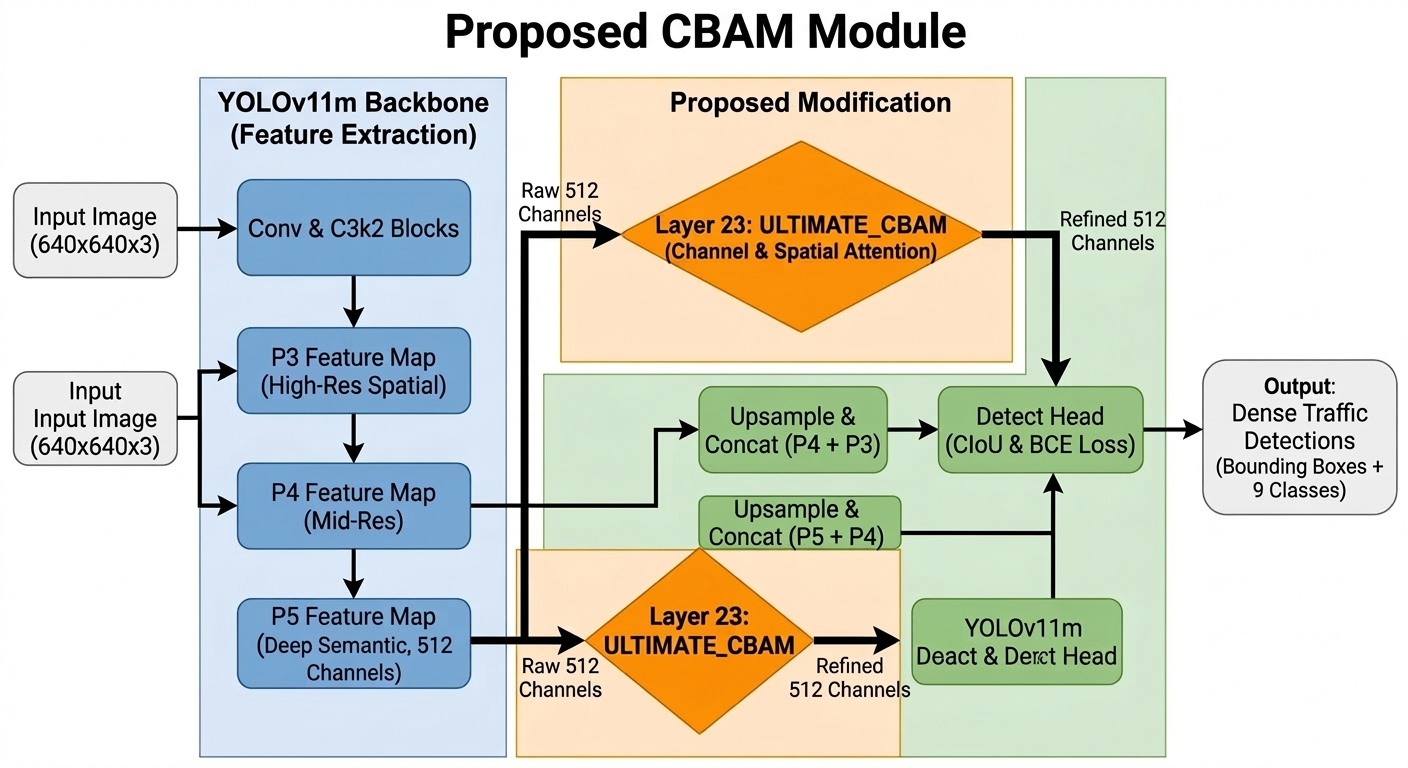
\includegraphics[width=0.9\linewidth]{Images/arch.png}
  \caption{Proposed attention-guided YOLOv11m architecture. The standard feature extraction backbone is modified by injecting a Convolutional Block Attention Module (CBAM) specifically at Layer~23. This intercepts the 512-channel P5 feature map prior to the detection head, applying sequential channel and spatial attention to filter background noise and emphasize the structural edges of highly occluded vehicles.}
  \Description{Diagram of the YOLOv11m network architecture showing feature flow from backbone to detection head, with CBAM sequential channel and spatial attention modules inserted at Layer 23 on the P5 feature map.}
  \label{fig:arch}
\end{figure}

\section{DATASET AND PREPROCESSING}
Collecting high-quality and properly annotated datasets is often challenging in many developing regions. Vehicles that are common in South Asian traffic, such as three-wheelers and various non-motorized transport, are rarely represented in widely used global datasets. For this reason, we created a custom dataset designed to reflect the real traffic conditions of Bangladesh in order to train our perception model.

\subsection{Data Sourcing and Curation}
We built our dataset by combining images collected from several regional traffic datasets. Most images collected from the Mendeley Bangladeshi Traffic Flow Dataset\cite{Islam2025BangladeshiTrafficFlow}. Extra images aded from the Dhaka-AI Dataset\cite{DVN/POREXF_2020} and Poribohon-BD Dataset\cite{19} to include more complex urban traffic scenes. Several preprocessing steps needed for the datasets before training the model. Few issues were annotations stored in XML and JSON formats and inconsistent bounding box coordinates in some subsets so we created a preprocessing script that parse annotations, clean incorrect values, and convert bounding box labels into normalized YOLO text format which makes a consistent dataset structure for training and evaluation. After preprocessing, the final dataset contains 23,648 images in total, including 18,919 images for training and 4,729 for validation. Across these images, we annotated 265,698 bounding boxes covering nine different vehicle classes commonly found in Bangladeshi traffic. To better understand how data availability affects model performance, we grouped the classes into three categories based on the number of instances in the dataset:

\begin{itemize}
    \item \textbf{Dominant Classes ($>$50,000 instances):} Car, Rickshaw, Bus
    \item \textbf{Mid-Tier Classes (10,000--50,000 instances):} People, CNG, Bike
    \item \textbf{Minority/Scarce Classes ($<$10,000 instances):} Mini-Truck, Truck, Cycle
\end{itemize}


The class distribution of the dataset is summarized in Table I and Fig.~\ref{fig:dataset_stats}. The numbers show a strong class imbalance in the collected traffic data. Vehicles such as cars and rickshaws appear far more frequently, while classes like cycles are much less common. In fact, the number of car instances is nearly 88 times higher than that of cycles.

\begin{table*}[htbp]
  \caption{Distribution of Classes in the Finalized Dataset}
  \label{tab:class_distribution}
  \begin{tabular}{llrrr}
    \toprule
    \textbf{Class Category} & \textbf{Vehicle Class} & \textbf{Train Instances} & \textbf{Validation Instances} & \textbf{Total Instances} \\
    \midrule
    Dominant 
     & Car        & 50,584  & 12,523 & 63,107  \\
     & Rickshaw   & 48,357  & 11,884 & 60,241  \\
     & Bus        & 41,573  & 10,423 & 51,996  \\
    \addlinespace
    Mid-Tier 
     & People     & 30,924  & 7,855  & 38,779  \\
     & CNG        & 22,356  & 5,467  & 27,823  \\
     & Bike       & 12,740  & 3,154  & 15,894  \\
    \addlinespace
    Minority 
     & Mini-Truck & 4,647   & 1,187  & 5,834   \\
     & Truck      & 1,009   & 301    & 1,310   \\
     & Cycle      & 566     & 148    & 714     \\
    \midrule
    \textbf{Total} & All Classes & 212,756 & 52,942 & 265,698 \\
    \bottomrule
  \end{tabular}
\end{table*}



\begin{figure}[h]
  \centering
  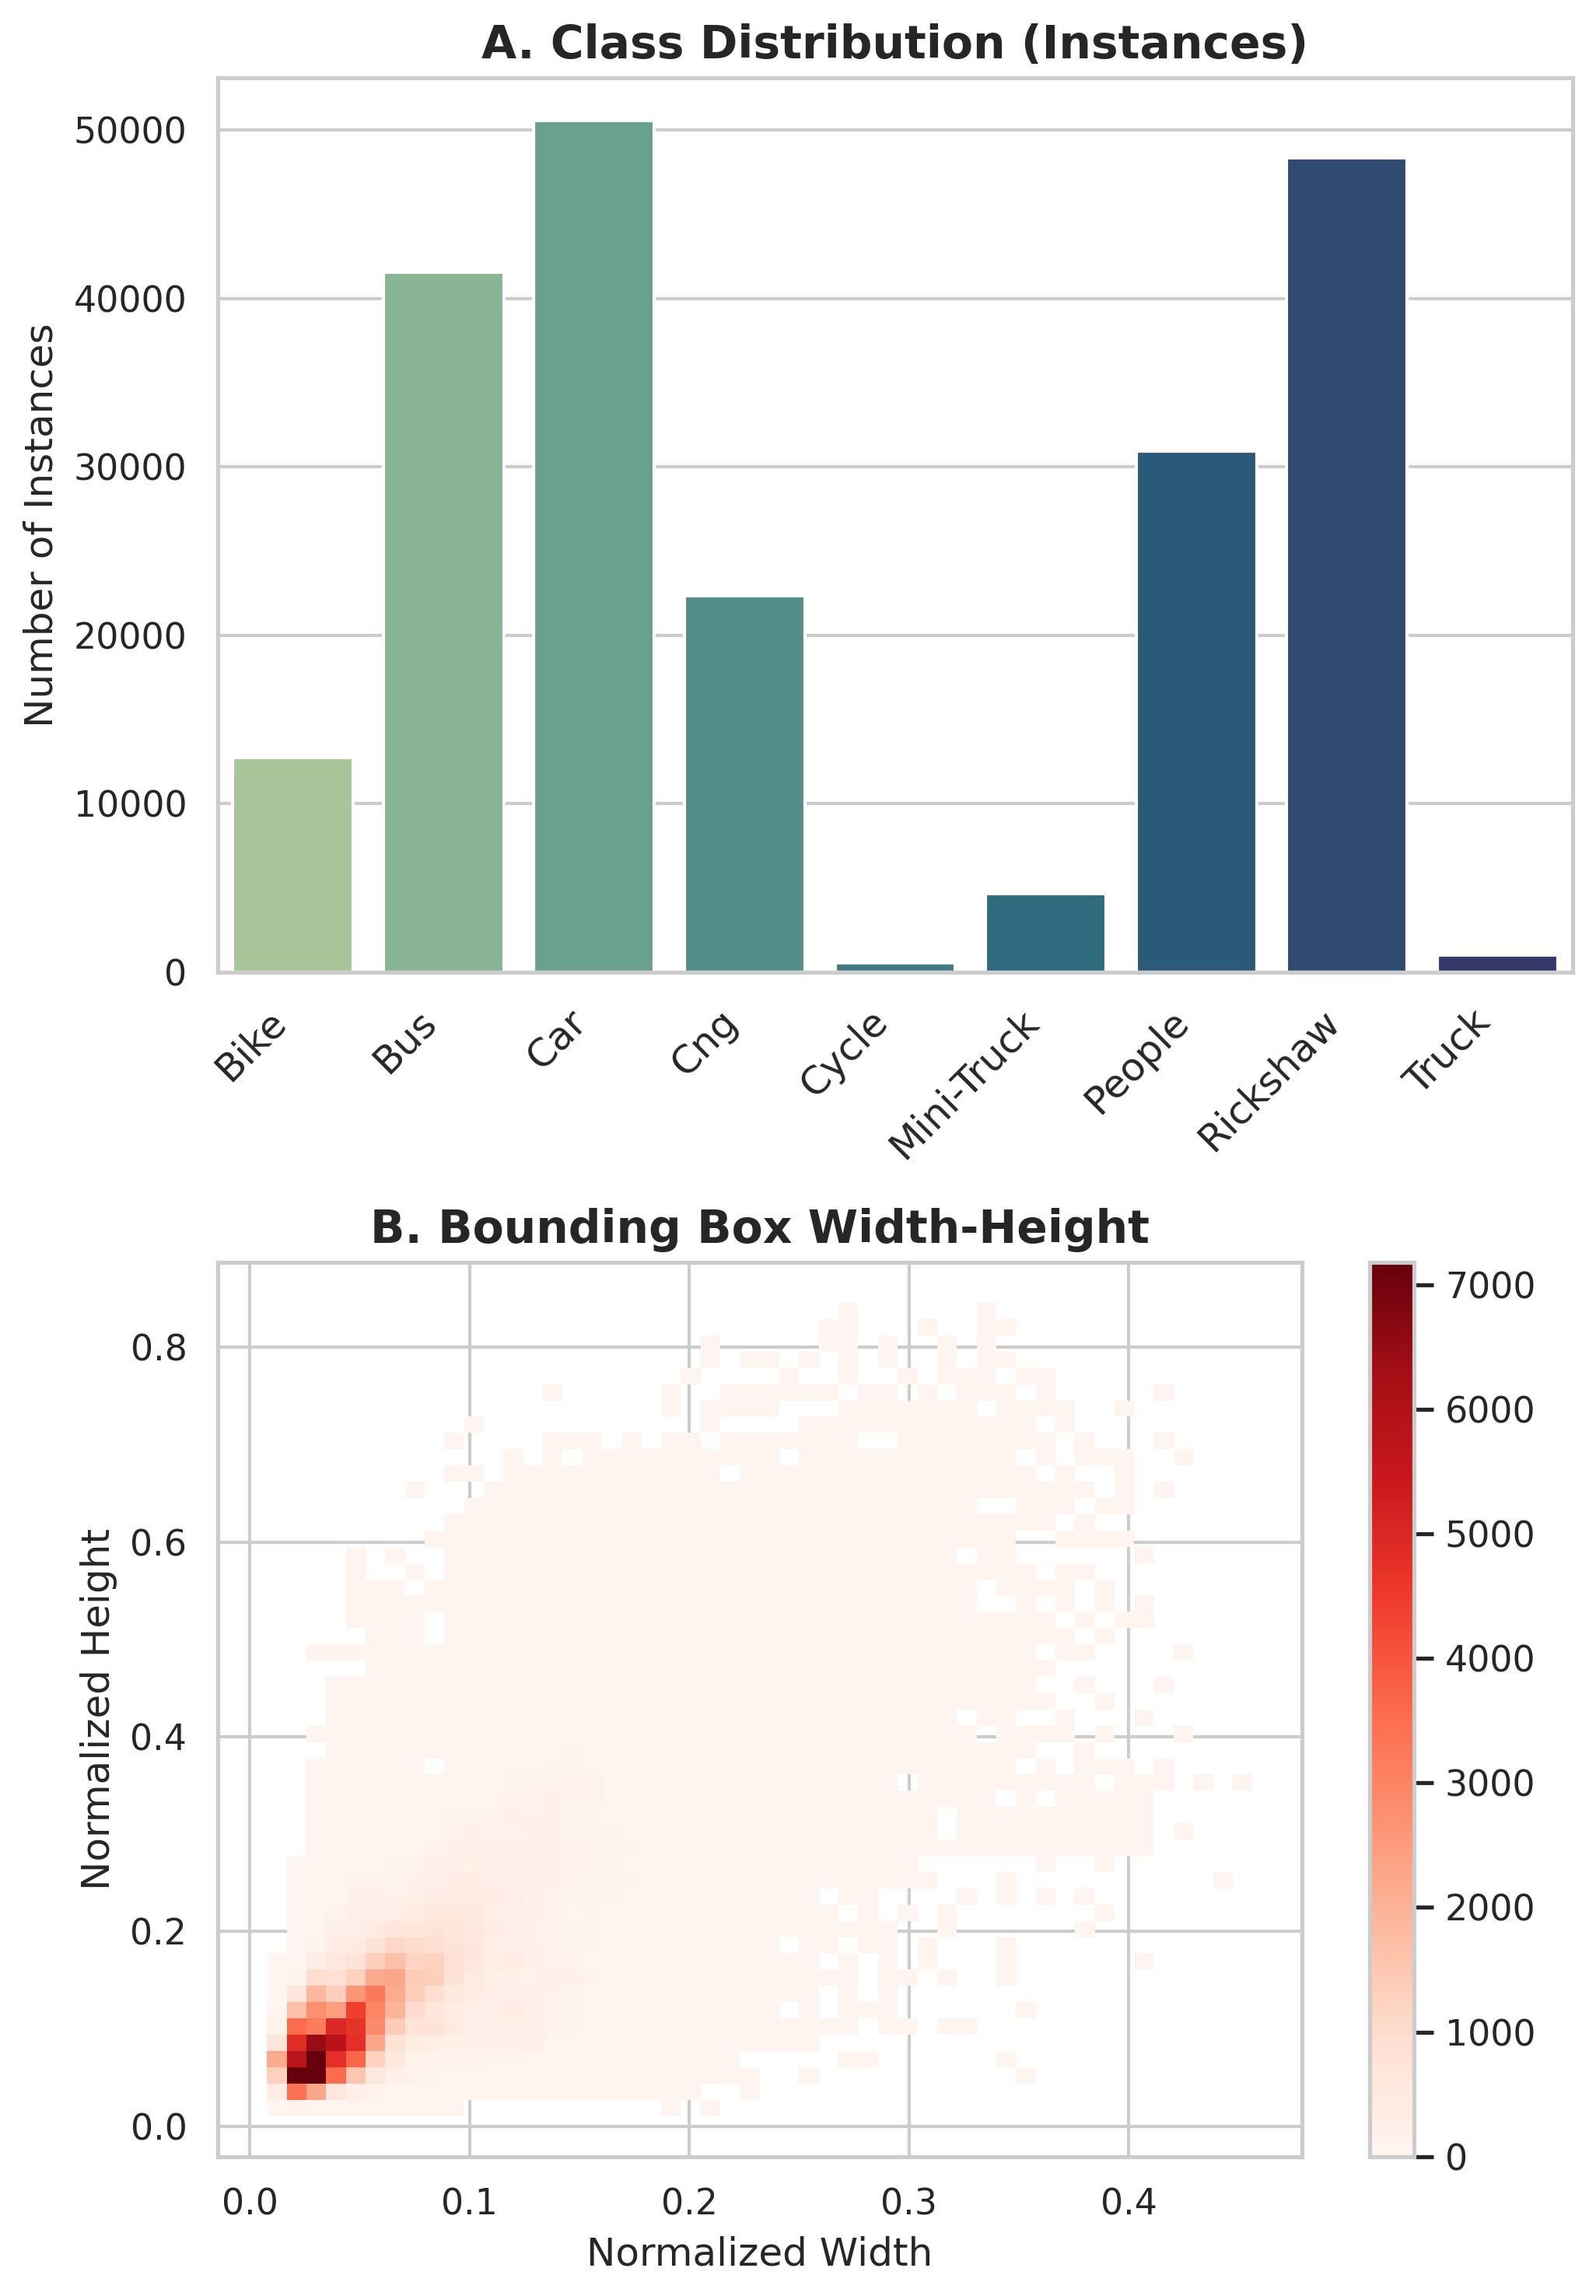
\includegraphics[width=\linewidth]{Images/IEEE_Single_Column_Stats.png}
  \caption{Dataset statistics and bounding box characteristics of the finalized \texttt{masterv1} dataset (265,698 instances). (A) The class distribution illustrates a severe long-tailed imbalance, dominated by structurally similar local vehicles like Cars and Rickshaws. (B) The bounding box density distribution confirms that the vast majority of detections possess extremely small spatial dimensions, simulating the dense occlusion characteristic of unstructured Dhaka traffic.}
  \Description{Two-panel statistical chart. Panel A is a bar chart showing class instance frequencies with dominant classes Car and Rickshaw. Panel B is a bounding box distribution density plot showing high concentration of small spatial boxes.}
  \label{fig:dataset_stats}
\end{figure}



\subsection{Advanced Augmentation Strategies}

Since the dataset contains a strong class imbalance, training the model with the original images alone can bias the model toward the dominant classes. To reduce this effect, we applied several data augmentation techniques during training using the Albumentations library. Specifically, we used Mosaic augmentation with a probability of 1.0, where four different images are combined into a single frame. This helps create crowded scenes and allows the model to learn from objects that are partially occluded. We applied an extra MixUp augmentation method that blends two images together with their corresponding labels. The MixUp approach helps the model to learn more stable features which reduces the chance of overfitting to dominant classes. 

\section{EXPERIMENTAL SETUP}

\subsection{Hardware and Configuration}

Baseline and modified models were trained with identical hyperparameters to ensure consistent evaluation and compared under the same setup for fairness, as summarized in Table~\ref{tab:param}. The models were trained in a cloud environment using dual NVIDIA Tesla T4 GPUs with 16GB VRAM each. 
\begin{table}[h]
  \centering
  \caption{Training Parameter Settings}
  \label{tab:param}
  \begin{tabular}{cll}
    \toprule
    \textbf{Sr. No.} & \textbf{Parameter} & \textbf{Value} \\ 
    \midrule
    1 & Training Epochs & 50 \\ 
    2 & Batch Size & 32 (distributed across dual \\ 
      &            & GPUs) \\ 
    3 & Optimizer & SGD (momentum = 0.937, \\ 
      &           & weight decay = 0.0005) \\ 
    4 & Initial Learning Rate & 0.01 \\ 
    5 & Learning Rate Scheduler & Cosine Annealing \\ 
    6 & Input Resolution & 640 $\times$ 640 pixels \\ 
    7 & Mixed Precision & Automatic Mixed Precision \\ 
      &                 & (AMP) Enabled \\ 
    \bottomrule
  \end{tabular}
\end{table}

\subsection{Evaluation Metrics}
The detection performance of the models is evaluated using standard Mean Average Precision (mAP) metrics. Specifically, we report mAP@0.50, which measures the average precision across all classes at a single Intersection over Union (IoU) threshold of 0.50, and mAP@0.50:0.95, which averages the mAP across ten IoU thresholds ranging from 0.50 to 0.95 with a step size of 0.05. In addition to detection accuracy, inference latency per frame (in milliseconds) is measured on the target GPU to assess real-time operational efficiency.


\section{RESULTS AND ANALYSIS}
To evaluate the performance of our approach in dense traffic scenes, we carried out two experiments. First, a standard YOLOv11m model was trained from scratch on our custom dataset to establish a baseline for Bangladeshi traffic conditions. Although the baseline model performed reasonably well, we observed that it often struggled to separate bounding boxes when vehicles were very close to each other. To address this limitation, we then trained our modified YOLOv11m+CBAM model, which is designed to better handle occlusion in crowded traffic scenes.

\subsection{Quantitative Performance}
When fully trained across 50 epochs, both architectures demonstrated stable convergence. As shown in Table~\ref{tab:ablation_overall}, our initial baseline YOLOv11m achieved a strong 75.1\% mAP@50. However, the introduction of the attention mechanism in our second experiment successfully pushed the overall validation performance to 75.7\% mAP@50.


\begin{table}[htbp]
  \caption{Overall Performance Comparison}
  \label{tab:ablation_overall}
  \begin{tabular}{lccc}
    \toprule
    \textbf{Architecture} & \textbf{mAP@0.50} & \textbf{mAP@0.50:0.95} & \textbf{Inference Speed} \\
    \midrule
    YOLOv11m baseline model       & 0.751 & 0.528 & $\sim$5.0 ms \\ 
    YOLOv11m integrated with CBAM & 0.757 & 0.532 & $\sim$4.7 ms \\
    \bottomrule
  \end{tabular}
\end{table}


Breaking down the 75.7\% overall performance by class (Table~\ref{tab:per_class_map}, Fig.~\ref{fig:per_class_ap_comparison}) reveals a massive contrast in how the attention mechanism handles structurally distinct vehicles versus minority classes heavily impacted by the dataset's long-tailed imbalance.

\begin{table}[htbp]
  \caption{Per-Class Average Precision (mAP@0.50)}
  \label{tab:per_class_map}
  \begin{tabular}{llcc}
    \toprule
    \textbf{Class Category} & \textbf{Vehicle Class} & \textbf{Baseline mAP@50} & \textbf{CBAM mAP@50} \\
    \midrule
    Dominant 
     & Car        & 0.934 & 0.934 \\
     & Rickshaw   & 0.905 & 0.908 \\
     & Bus        & 0.892 & 0.894 \\
    \addlinespace
    Mid-Tier 
     & People     & 0.866 & 0.868 \\
     & CNG        & 0.910 & 0.911 \\
     & Bike       & 0.837 & 0.846 \\
    \addlinespace
    Minority 
     & Mini-Truck & 0.655 & 0.666 \\
     & Truck      & 0.455 & 0.470 \\
     & Cycle      & 0.305 & 0.316 \\
    \bottomrule
  \end{tabular}
\end{table}

\begin{figure}[htbp]
  \centering
  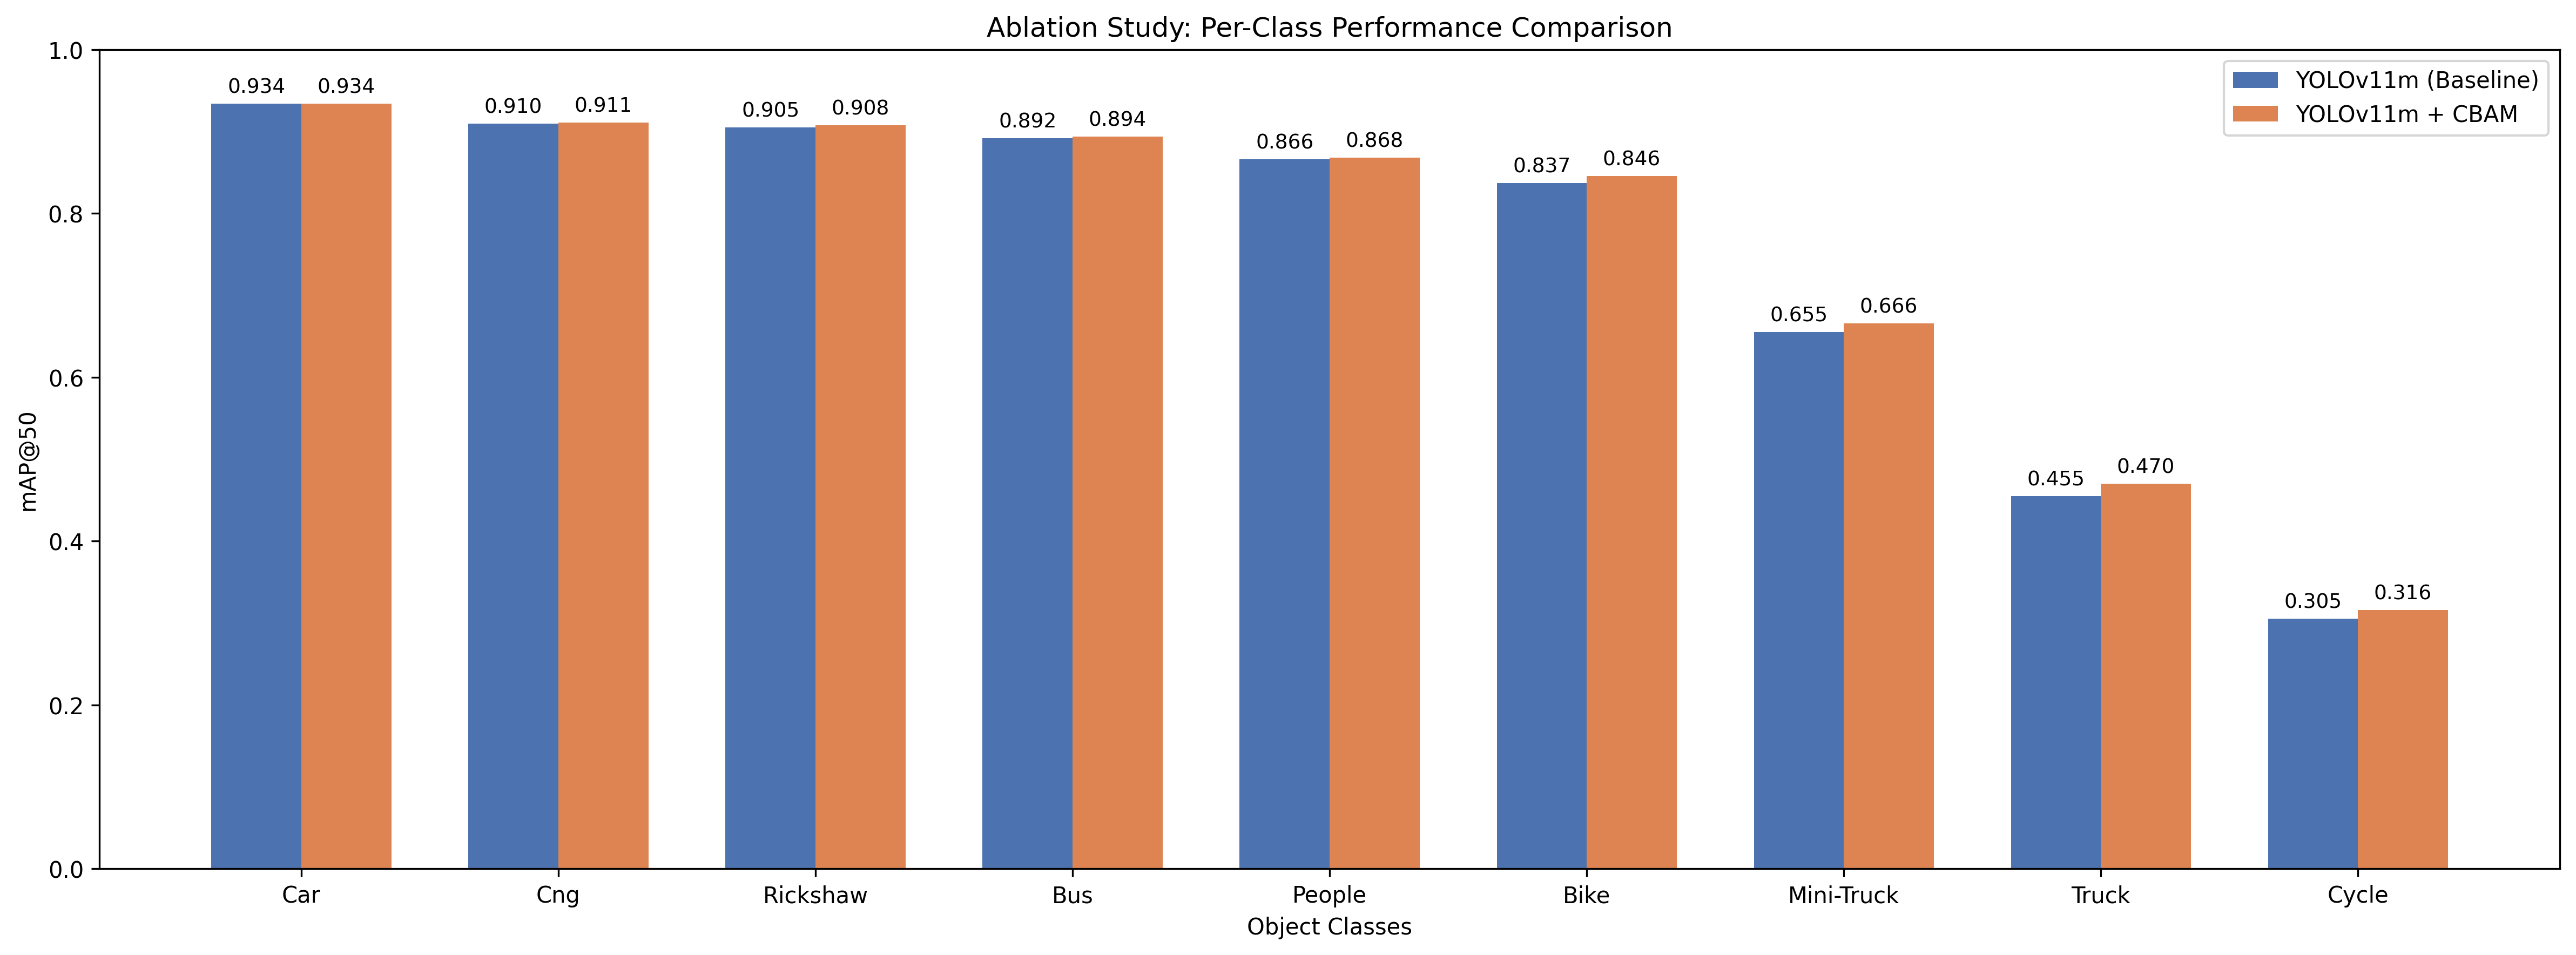
\includegraphics[width=\linewidth]{Images/ablation_study_map50.png}
  \caption{Comparative study of per-class Average Precision (mAP@0.50). While our baseline model established strong initial metrics, the proposed YOLOv11m+CBAM architecture successfully extracted obscured features in heavily occluded minority classes, yielding significant AP gains for Trucks (+1.5\%) and Mini-Trucks (+1.1\%).}
  \Description{Comparative horizontal bar chart showing per-class mAP at 0.50 for baseline YOLOv11m versus YOLOv11m plus CBAM across all nine vehicle classes, highlighting improvements on minority classes.}
  \label{fig:per_class_ap_comparison}
\end{figure}

The data confirms our hypothesis. For heavily represented classes like Cars, CNGs, and Rickshaws, the baseline model was already highly capable, pushing past 90\% AP. However, the standard convolutional layers failed on structurally distinct minority classes. By adding spatial and channel attention mechanisms, our second model provided noticeable AP improvements ($>1.0\%$) for Trucks, Mini-Trucks, and Cycles, which we attribute to the attention mechanism helping the network emphasize informative spatial and channel features of minority vehicles amid complex backgrounds.

\subsection{Computational Overhead}

A common drawback of adding attention modules is a loss of processing speed. To validate that our high accuracy was achieved without sacrificing operational viability, we benchmarked both of our models. Our initial baseline processed images at roughly 5.0ms per frame. Remarkably, our custom YOLOv11m+CBAM architecture maintained an exceptional 4.7ms inference speed on the Tesla T4. This proves that integrating CBAM deep within the backbone substantially boosts perception accuracy in heavy occlusion without introducing computational latency, perfectly preserving real-time capability for edge-device ADAS deployment.

\section{DISCUSSION AND ERROR ANALYSIS}
The YOLOv11m+CBAM model performs better in dense traffic scenes but many challenges remain including class imbalance, structural confusion between visually similar vehicles, and difficulties in detecting sparse or occluded objects. The following subsections issues each in detail.

\subsection{Class Imbalance and Detection Performance}

After training the model, it shows a clear pattern in the performance across different vehicle categories. The model performs very well on classes such as cars, rickshaws, buses, and CNGs, achieving high detection accuracy because of the high amount of data for these particular classes. On the other hand, the performance dropped significantly when identifying the minority classes, such as cycles and trucks. This indicates that the model is highly influenced by the distribution of training data. For better performance, it requires sufficient training of the model. The model achieves strong detection performance when only a large number of training samples are available for categories. Vehicles like cars, rickshaws, and buses appear frequently in the dataset, which allows the model to learn structural patterns more effectively. Additionally, these vehicles have distinct shapes and strong visual features, that's why it is easier for a convolutional neural network to detect them properly even in dense traffic areas. The model struggled to detect cycles because bicycles have very thin structural features. Another factor is dataset imbalance, as the number of cycle instances in the dataset is extremely low compared to other dominant classes. In many cases, the model focuses on the rider instead of the bicycle, which results in misclassification as a pedestrian.

\subsection{Class-Wise Performance Disparities}
As reflected in the evaluation, Truck detection proves more challenging than dominant categories such as Bus. Table~\ref{tab:class_distribution} shows that Truck has substantially fewer instances than Bus, and Table~\ref{tab:per_class_map} reports lower per-class AP for Truck than Bus, indicating that class imbalance may contribute to this performance difference. The dataset follows a long-tailed distribution where dominant classes have thousands of instances, but minority classes contain only a few hundred samples. As reflected in Table~\ref{tab:class_distribution} and Table~\ref{tab:per_class_map}, heavily represented classes achieve high detection performance, whereas minority categories have substantially fewer training instances and lower reported Average Precision.

\subsection{Qualitative Performance}

We checked predictions from the validation dataset to better understand the model behavior. As shown in Fig.~\ref{fig:qualitative_results} the architecture produces tight and well-separated bounding boxes, even in dense traffic. In crowded scenes, the detector correctly identifies overlapping vehicles like cars, rickshaws and buses. By integrating CBAM attention module helps the network to focus on spatial and channel features, reducing suppression issues and improves consistent detection in complex environments, especially with occlusion and clutter.

\begin{figure}[htbp]
  \centering
  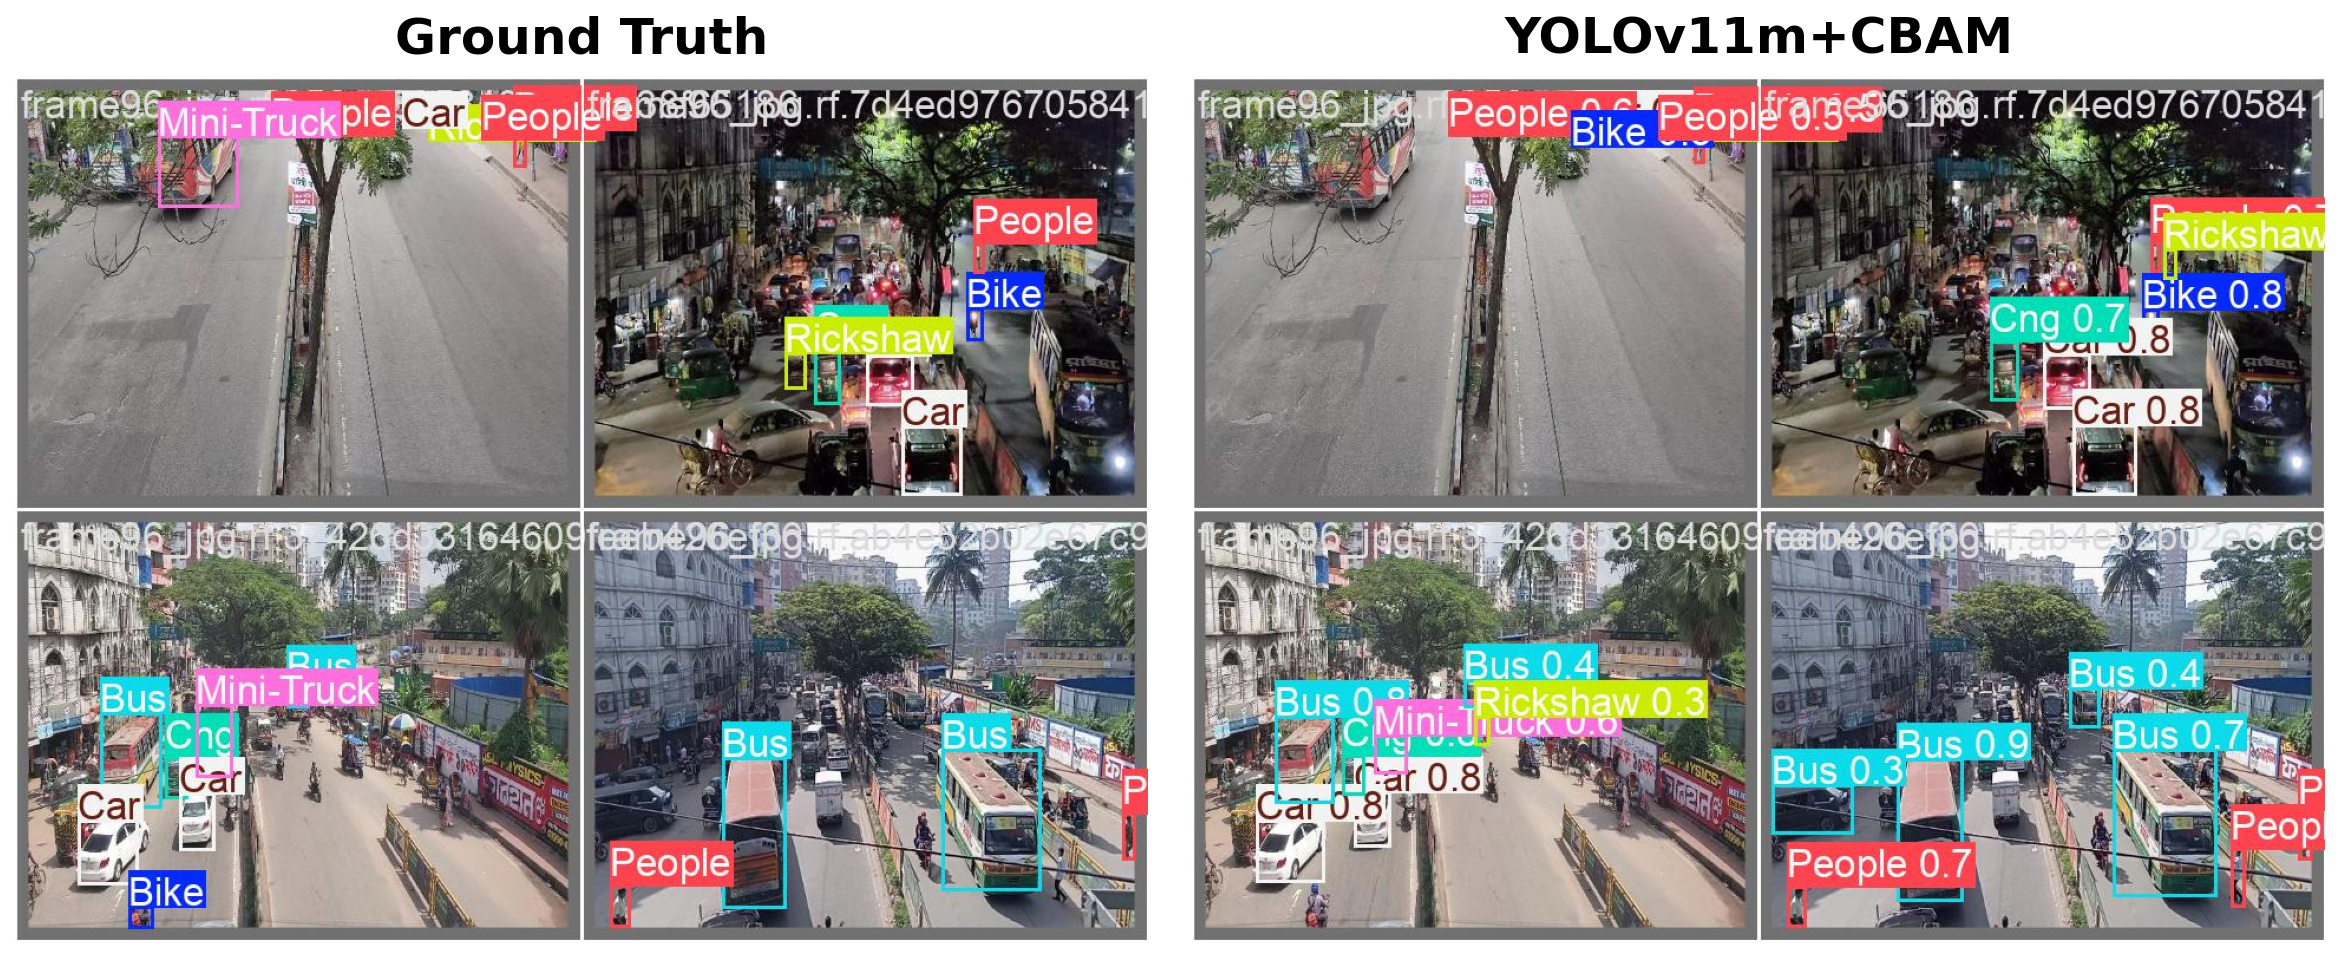
\includegraphics[width=\linewidth]{Images/IEEE_Qualitative_Results.png}
  \caption{Qualitative detection results on the validation set. Left: ground truth annotations. Right: predictions from the YOLOv11m+CBAM model in dense unstructured traffic.}
  \Description{Photographic qualitative comparison showing four urban traffic scenes with ground truth bounding boxes on the left and YOLOv11m plus CBAM model predictions on the right.}
  \label{fig:qualitative_results}
\end{figure}

However, the qualitative results also reveal limitations and some challenges still remain. The model still struggles with sparse structural objects such as cycles, especially when only a limited number of training samples are available. In addition, vehicles with similar visual structures, such as trucks and buses, remain difficult to distinguish when their visual features appear very similar. These observations indicate that architectural improvements alone may not fully solve the problem. Future work should therefore focus on improving dataset balance and collecting more samples for minority vehicle classes.

\section{CONCLUSION AND FUTURE WORK}
The main objective of this research was to improve object detection in unstructured Bangladeshi traffic environments by developing an attention-guided detection model. A large unified dataset was created by merging multiple regional datasets. To improve feature extraction in dense and occluded traffic scenes, a modified YOLOv11m architecture integrated with the Convolutional Block Attention Module (CBAM) was presented. The experimental results showed that the baseline model achieved 75.1\% mAP@50, while the proposed YOLOv11m+CBAM model improved performance to 75.7\% mAP@50. The model performs well on local vehicle classes such as Rickshaws and CNGs, achieving per-class Average Precision above 90\% at IoU 0.50. These results are significant for Intelligent Transportation Systems (ITS) and Advanced Driver Assistance Systems (ADAS) in developing countries, aiding road safety, traffic monitoring, and autonomous driving technology. Nevertheless, the model still faces limitations due to severe class imbalance for minority classes such as cycles and trucks. Future research will focus on addressing this dataset imbalance problem.

%%
%% The next two lines define the bibliography style to be used, and
%% the bibliography file.
\bibliographystyle{ACM-Reference-Format}
\bibliography{rf}

\end{document}
\endinput
%%
%% End of file `main_template_based.tex'.
